% PGF text plot marks used to annotate force-vector endpoints.
\documentclass[border=2pt]{standalone}
\usepackage{tikz}
\usetikzlibrary{arrows.meta,plotmarks}

\begin{document}
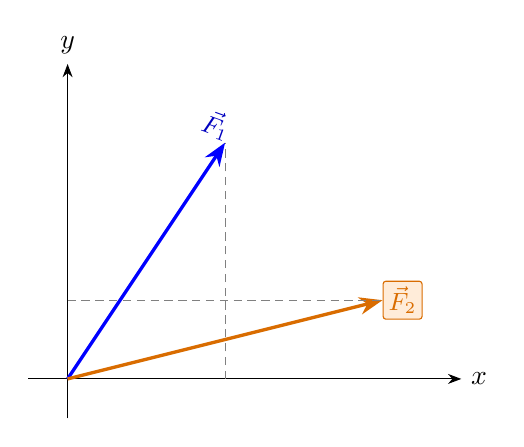
\begin{tikzpicture}[>=Stealth]
  \draw[->] (-0.5,0) -- (5,0) node[right] {$x$};
  \draw[->] (0,-0.5) -- (0,4) node[above] {$y$};
  \draw[very thick,blue,-Stealth] (0,0) -- (2,3);
  \draw[very thick,orange!85!black,-Stealth] (0,0) -- (4,1);
  \draw[densely dashed,gray] (2,0) -- (2,3);
  \draw[densely dashed,gray] (0,1) -- (4,1);
  \draw[blue!75!black]
    plot[mark=text,text mark={{\small$\vec F_1$}},
      text mark style={bottom,right,rotate=-20}]
    coordinates {(2,3)};
  \draw[orange!85!black]
    plot[mark=text,text mark={$\vec F_2$},text mark as node=true,
      text mark style={draw,fill=orange!15,rounded corners=1pt,inner sep=2pt,font=\small,anchor=west}]
    coordinates {(4,1)};
\end{tikzpicture}
\end{document}
